\documentclass{article}
\usepackage{pgfplots}
\pgfplotsset{compat=1.9}
\usepackage{tikz}
\usetikzlibrary{positioning}
\usetikzlibrary{backgrounds}

\begin{document}
	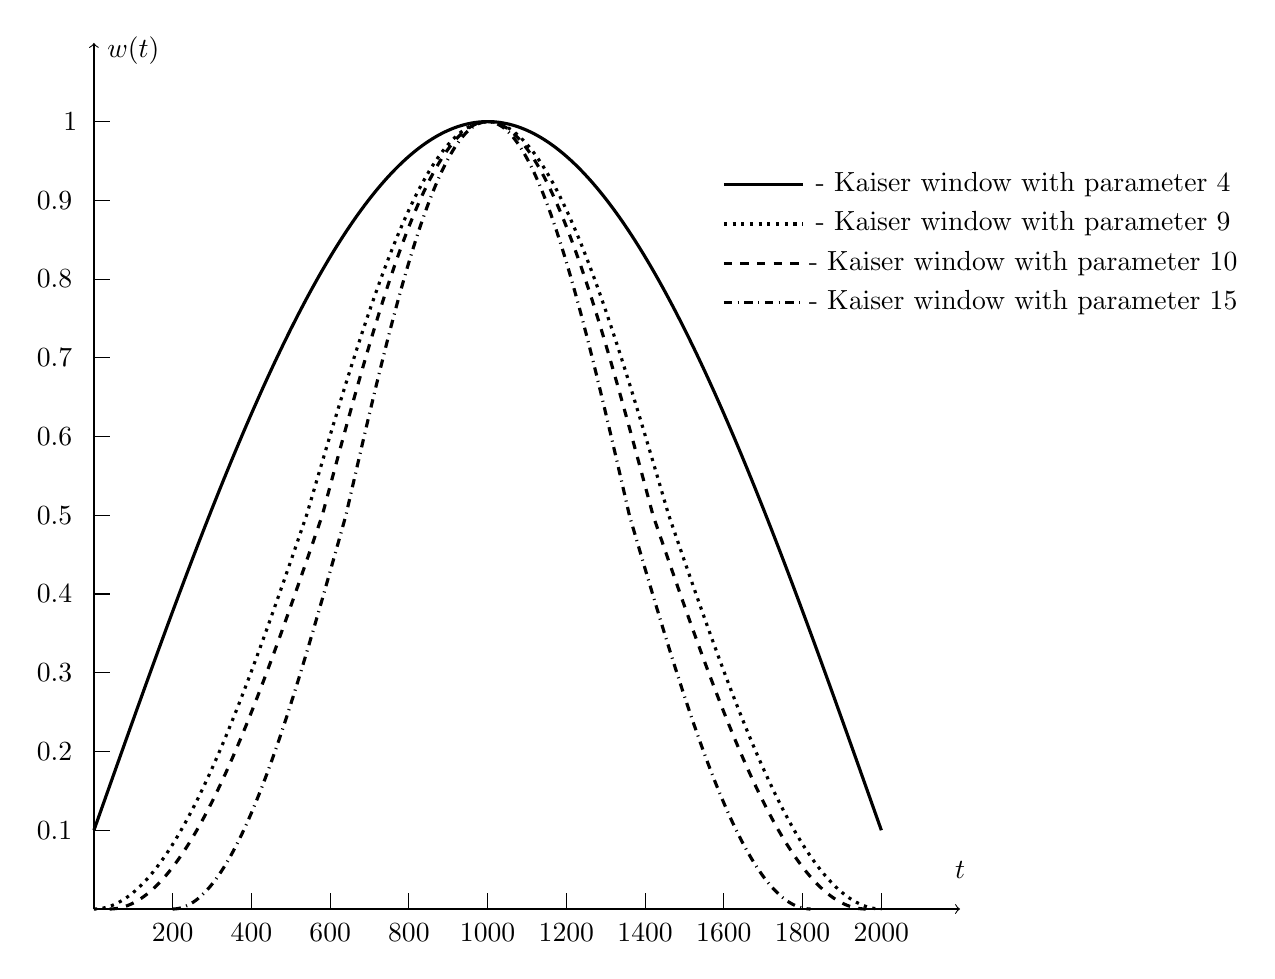
\begin{tikzpicture}
	\draw[->] (0,0) -- (11,0);
	\foreach \x in {1,2,...,10} {
	\draw (\x,0) -- (\x,.2);
}
	\draw[->] (0,0) -- (0,11); %9.8
	\foreach \y in {1,2,...,10} {
	\draw (0,\y) -- (.2,\y);
}
	%grap
	\draw[line width=.4mm] (0,1) sin (5,10) cos (10,1);
	\draw[dotted,line width=.4mm] (0,0) cos (2.7,5) sin (5,10) cos (7.3,5) sin (10,0);
	\draw[dashed,line width=.4mm] (.2,0) cos (2.9,5) sin (5,10) cos (7.1,5) sin (9.8,0);
	\draw[dashdotted,line width=.4mm] (1,0) cos (3.2,5) sin (5,10) cos (6.8,5) sin (9.1,0);
	
	\node () at (1,-0.3) {200};
	\node () at (2,-0.3) {400};
	\node () at (3,-0.3) {600};
	\node () at (4,-0.3) {800};
	\node () at (5,-0.3) {1000};
	\node () at (6,-0.3) {1200};
	\node () at (7,-0.3) {1400};
	\node () at (8,-0.3) {1600};
	\node () at (9,-0.3) {1800};
	\node () at (10,-0.3) {2000};
	
	\node () at (-.5,1) {0.1};
	\node () at (-.5,2) {0.2};
	\node () at (-.5,3) {0.3};
	\node () at (-.5,4) {0.4};
	\node () at (-.5,5) {0.5};
	\node () at (-.5,6) {0.6};
	\node () at (-.5,7) {0.7};
	\node () at (-.5,8) {0.8};
	\node () at (-.5,9) {0.9};
	\node () at (-.3,10) {1};
	
	\node () at (.5,10.9) {$w(t)$};
	\node () at (11,.5) {$t$};
	
	\draw[dashdotted,line width=.4mm] (8,7.7) -- (9,7.7);
	\draw[dashed,line width=.4mm] (8,8.2) -- (9,8.2);
	\draw[dotted,line width=.4mm] (8,8.7) -- (9,8.7);
	\draw[line width=.4mm] (8,9.2) -- (9,9.2);
	
	\node () at (11.8,7.7) {- Kaiser window with parameter 15};
	\node () at (11.8,8.2) {- Kaiser window with parameter 10};
	\node () at (11.8,8.7) {- Kaiser window with parameter 9};
	\node () at (11.8,9.2) {- Kaiser window with parameter 4};
	\end{tikzpicture}
\end{document}